% Created 2018-07-11 Wed 15:30
% Intended LaTeX compiler: pdflatex
\documentclass[11pt]{article}
\usepackage[utf8]{inputenc}
\usepackage[T1]{fontenc}
\usepackage{graphicx}
\usepackage{grffile}
\usepackage{longtable}
\usepackage{wrapfig}
\usepackage{rotating}
\usepackage[normalem]{ulem}
\usepackage{amsmath}
\usepackage{textcomp}
\usepackage{amssymb}
\usepackage{capt-of}
\usepackage{hyperref}
\date{\today}
\title{}
\hypersetup{
 pdfauthor={},
 pdftitle={},
 pdfkeywords={},
 pdfsubject={},
 pdfcreator={Emacs 26.0.91 (Org mode 9.1.13)}, 
 pdflang={English}}
\begin{document}

\tableofcontents

\section{Finanzmanagement}
\label{sec:orgbeea28e}
Funktion des Finanzmanagement ist die zielgerichtete Gestaltung der betrieblichen Finanzwirtschaft:
\begin{itemize}
\item aktive Gestaltung der Kapitalzuführung und des Kapitalentzugs
\item eher passive Gestaltung der internen Finanzbewegungen
\item bezeichnet auch die mit den Managementaufgaben Finanzierung \& Finanzwirtschaft verantwortlich betrauten Mitglieder einer Organisation
\end{itemize}
\subsection{Finanzierung \& Wettbewerbsfähigkeit}
\label{sec:orgc0c8d92}
Ziel der Finanzwirtschaft ist die Erreichung des finanzwirtschaftlichen Gleichgewichts
\subsubsection{Zahlungsstrom, Finanzierungsmaßnahme, Kapitalveränderung}
\label{sec:orga3dc6b1}
\begin{itemize}
\item \textbf{klassischer Kapitalbegriff} = Kapital ist die abstrakte Wertsumme der Bilanz; Kapital zeigt die Herkunft der Werte des Unternehmens an, unterteilt in Eigen- und Fremdkapital
\item \textbf{monetärer Kapitalbegriff} = Kapital sind im Unternehmen eingesetzte Geldmittel
\end{itemize}

Finanzwirtschaft umfasst die Kapitalbeschaffung und -verwendung der Unternehmung

\begin{enumerate}
\item Kapitalströme
\label{sec:orgfa6f9f6}
\begin{figure}[htbp]
\centering
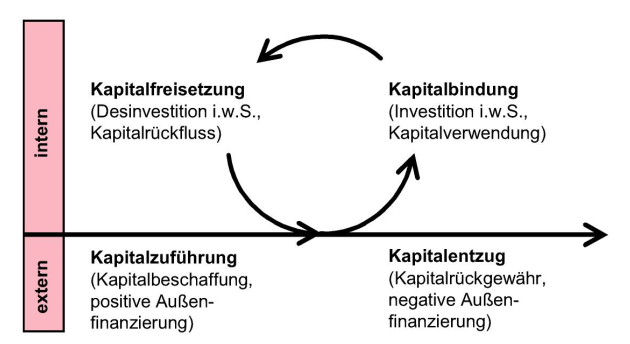
\includegraphics[width=250px]{./pictures/kapitalstroeme.png}
\caption{Kapitalveränderung als Strömungsgröße}
\end{figure} 
\begin{itemize}
\item Kapitalbindung (oder -verwendung)
\item Kapitalfreisetzung (oder -rückfluss)
\item Kapitalzuführung (oder -beschaffung)
\item Kapitalentzug (oder -abfluss)
\end{itemize}

\item Finanzielles Gleichgewicht
\label{sec:org4cd7195}
\begin{figure}[htbp]
\centering
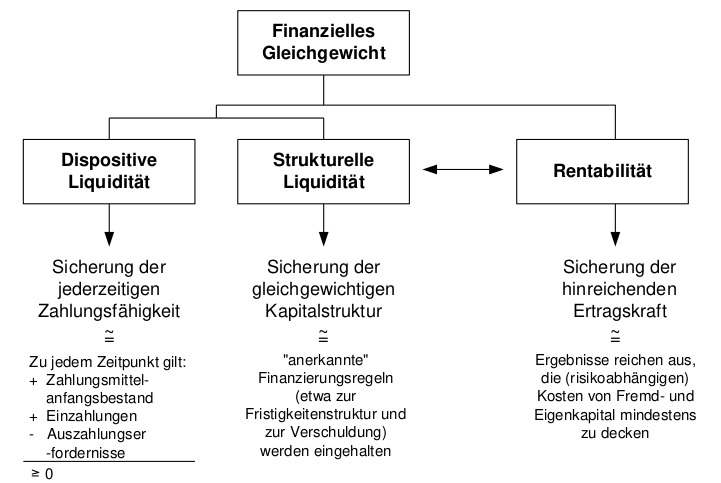
\includegraphics[width=250px]{./pictures/finanzgg.png}
\caption{Komponenten des finanziellen Gleichgewichts}
\end{figure}
\end{enumerate}
\subsubsection{Zahlungsbeziehungen, Finanzierungsform, Finanzierungsverträge}
\label{sec:org9e15863}
\begin{enumerate}
\item Zahlungsbeziehungen
\label{sec:org2fe2e36}
F.14 II\(_{\text{FInanzmnfgm}}\)\(_{\text{1.pdf}}\)
\item Herkunft von Finanzmitteln
\label{sec:org23a87da}
\textbf{Außenfinanzierung} \(\rightarrow\) = \textbf{Kapitalzuführung}
\begin{itemize}
\item finanzielle Mittel oder geldwertäquivalente Vermögensgegenstände werden dem Unternehmen \emph{explizit} von auf Finanzierungsmärkten (also \emph{außerhalb}) operierenden Financiers zur Verfügung gestellt
\begin{itemize}
\item Geldmarkt: Finanzmittel mit kurzer Laufzeit (zB Bank-, Kunden-, Lieferantenkredite)
\item Kapitalmarkt: Finanzmittel mit mittlerer \& längerer Laufzeit (zB Darlehen, Hypotheken, Anleihungen, Beteiligungen)
\end{itemize}
\end{itemize}

\textbf{Innenfinanzierung} \(\rightarrow\) = \textbf{Kapitalfreisetzung}
\begin{itemize}
\item finanzielle Mittel die dem Unternehmen in Form eines (positiven) Saldos zwischen Einzahlungen aus Nicht-Finanzierungsmärkten \& Auszahlungen an diese Märkte in einer Periode zugeflossen sind, werden am Verlassen des Unternehmens gehindert (\emph{innerhalb})
\begin{itemize}
\item der finanz. Überschuss wird als Cash-Flow bezeichnet und drückt die Innenfinanzierung eines Unternehmens aus
\end{itemize}
\end{itemize}
\item Finanzierungsverträge
\label{sec:orgb5bf5fd}
Ein Finanzierungsvertrag hält die Bedingungen fest zu denen ein Unternehmen finanzielle Mittel beschafft:
\begin{itemize}
\item Höhe \& Zeitpunkt
\item Sicherheitsgrad der Zahlungen
\end{itemize}

Es gibt 3 Formen von Finanzierungsverträgen:

\begin{enumerate}
\item Unbedingter Finanzierungsvetrag
Das Unternehmen leistet bestimmte, vertragliche fixierte Zins- und Tilgungszahlungen immer \& unter allen Umständen an den Geldgeber (zB standardisierter Kreditvertrag)

\item Bedingter Finanzierungsvertrag
Das Unternehmen leistet präzisierte Zahlungen an den Geldgeber, wenn bestimmte Bedingungen erfüllt sind (zB positiver Jahresabschluss bei Gewinnobligationen, Genussscheinen, Stamm- oder Vorzugsaktion)

\item Sicherungsvertrag
Das Unternehmen vereinbart Maßnahmen zur Besicherung der Finanzierungsmaßnahme sowie zu Informations- und Kontrollrechten des Geldgebers
\end{enumerate}
\end{enumerate}

\subsubsection{Optimale Finanzierung \& Wettbewerbsfähigkeit}
\label{sec:orgf4a526b}
Es gibt Probleme beim Erreichen des Ziels der optimalen Finanzierung. Die Konsequenzen von Investitionsprogrammen \& Finanzierungsverträgen sind für Eigentümer \& Gläubiger nicht vollständig bekannt, außerdem sind ihre Erwartungen unterschiedlich. Finanzierung kann außerdem Hinblick auf verschiedene andere Ziele/Faktoren betrachtet werden:

\begin{enumerate}
\item Finanzierung \& Liquidität
Sicherung der Zahlungsfähigkeit innerhalb eines gegebenen Planungszeitraums

\item Finanzierung \& Rentabilität
Konsistente Aussagen zum erwarteten Erfolg investierter Mittel / im Vergleich von Planungszeitraum / ggü dem Kapitalmarkt

\item Finanzierung \& Risiko
Prognose des Eintritts des erwarteten Erfolgs investiertet Mittel (Eintrittswahrscheinlichkeit) / Finanzierungsverträge zur Risikoteilung bei Eigen- und Fremdfinanzierung
\end{enumerate}

II\(_{\text{Finanzmanagement}}\)\(_{\text{2.pdf}}\) -> F.6 Zusammenfassung

\subsection{Bereitstellung finanzieller Ressourcen}
\label{sec:orge2894b1}
\subsubsection{Formen der Finanzierung}
\label{sec:org2d10dfa}
\begin{center}
\begin{tabular}{lll}
Herkunft der Finanzmittel/Rechtsstellung des Kapitalgebers & Eigenfinanzierung (Eigentümer) & Fremdfinanzierung (Gläubiger)\\
\hline
Außenfinanzierung & Beteiligungsfinanzierung & Kreditfinanzierung\\
Innenfinanzierung & Selbstfinanzierung (insbs. aus Gewinnen) & Sonstige (insbs. Rückstellungen)\\
\end{tabular}
\end{center}

\textbf{Beteiligungsfinanzierung} = Finanzierung durch (bisherige oder neue) Eigentümer
\begin{itemize}
\item Eigenkapital (von außen zugeführt oder entsprechende Sacheinlagen der Eigentümer)
\item Beteiligungskapital
\begin{itemize}
\item Beschaffung von Eigenkapital durch Aufnahme neuer Teilhaber (Gesellschafter) bei nicht emissionsfähigen Unternehmen
\item Beschaffung von Eigenkapital bei emissionfähigen Unternehmen (Stammaktie/Vorzugsaktie/Genussschein)
\end{itemize}
\end{itemize}

\textbf{Kreditfinanzierung} = Finanzierung durch externe Kapitalgeber (Gläubiger)
\begin{itemize}
\item Formen der langfristigen Kreditfinanzierung über den Kapitalmarkt
\begin{itemize}
\item Schuldverschreibung, Industrieanleihe
\item Schuldscheindarlehen, Investitionsdarlehen
\end{itemize}
\item Formen der kurzfristigen Kreditfinanzierung über den Geldmarkt
\begin{itemize}
\item Bank-/Handels-/Lieferantenkredite
\end{itemize}
\item Sonderformen
\begin{itemize}
\item Factoring, Leasing
\end{itemize}
\end{itemize}

\begin{center}
\begin{tabular}{lll}
Vergleichskriterium & Beteiligungsfinanzierung & Kreditfinanzierung\\
\hline
Anspruchsgrundlage & Quotenanteil & Nominalanspruch\\
Erfolgsansrpuch & erfolgsabhängig/variabel & erfolgsunabhängig/kontraktbestimmt\\
Befristung & Nein & Ja\\
Haftung & Ja zumindest begrenzt & Nein\\
Leitung & Ja zumindest begrenzt & Nein\\
\end{tabular}
\end{center}

\begin{enumerate}
\item Wahl der optimalen Finanzierung
\label{sec:org23725c1}
\textbf{Finanzierung \& Risiko/Chance}
\begin{itemize}
\item Financiers werden - unter sonst gleichen Bedingungen - eine Finanzierung umso besser einschätzen, je sicherer die in Aussicht gestellten Renditen sind
\begin{itemize}
\item Risiko/Chance kann gleichgesetzt werden mit der Möglichkeit des Eintreten eines ggü dem Erwartungswert nachteiligen/vorteilhaften finanz. Ereignisses/Ergebnisses
\item Risiko/Chance liegt dann vor, wennn eine eingetretene Nettoeinzahlung (finanzielles Ergebnis) unterhalb/oberhalb des eingesetzten Kapitals liegt
\end{itemize}
\end{itemize}

\textbf{Liquidität (finanz. Gleichgewicht)}
\begin{itemize}
\item ein Unternehmen ist liquide (zahlungsfähig), wenn es in der Lage ist, seinen Zahlungsverpflichtungen innerhalb eines gegebenen Planungszeitraums jederzeit vertragskonform nachzukommen
\begin{itemize}
\item Zahlungsfähigkeit = Zahlungsvermögen > Zahlungsverpflichtungen
\end{itemize}
\item \emph{Risiko der Liquidität}: Aufrechterhaltung der Liquidität ist eine notwendige Voraussetzung für den Fortbestand eines Unternehmens. Aktuelle oder drohende Zahlungsunfähigkeit oder eine Überschuldung sind Gründe für eine Insolvenz
\end{itemize}

\textbf{Rentabilität}
\begin{itemize}
\item Rentabilität spiegelt das Ergebnis unternehmerischer Tätigkeit wieder, in dem der finanzwirtsch. Erfolg in Relation zum eingesetzten Kapital gesetzt wird 
\begin{itemize}
\item Eigenkapital, Gesamtkapital, Umsatz
\end{itemize}
\item \emph{Risiko der Rentabilität}: zur zukunftsgerichteten Begründung von Entscheidung ist mit Erwartungswerten zu rechnen, die an Bedeutung verlieren, je größer die Unsicherheit ist
\end{itemize}
\end{enumerate}

\subsection{Finanzierungsplanung}
\label{sec:org4d55d98}
\begin{enumerate}
\item Begriff \& Arten der Liquidität
\label{sec:org2070e5e}
Ein Unternhemen ist \emph{liquide} (zahlungsfähig), wenn es in der Lage ist, seinen Zahlungsverpflichtungen innerhalbs eines gegebenen Planungszeitraums jederzeit vertragskonform nachzukommen. Die Aufrechterhaltung der Liquidität ist eine notwendikge Voraussetzung für den Fortbestand eines Unternehmens. Aktuelle oder drohende Zahlungsunfähigkeit oder eine Überschuldung sind Gründe für eine Insolvenz.

Arten der Liquidität:
\begin{itemize}
\item güterwirtschaftliche Liquidät
\item verliehende Liquidität
\item zukünftige Liquidität
\item antizipierte Liquidität
\end{itemize}

Messung von Liquidität:
\begin{itemize}
\item Beurteilung anhand der Liquiditätsgrade \& der Struktur von Kapitalbindung und -bereitstellung (horizontale Kapitalstruktur = Vergleich von Vermögen und Kapitalstruktur), sowie anhand des Verschuldungsgrads (vertikale Kapitalstruktur = Vergleich von Eigen- und Fremdkapital)
\item Beurteilung auf der Basis von Finanzplänen
\end{itemize}

II\(_{\text{Finanzmanagement}}\)\(_{\text{2.pdf}}\) F.22 Zusammenfassung
\end{enumerate}
\end{document}
